\documentclass[../TDM3_courbe_app.tex]{subfiles}%

\begin{document}
\section[s]"1"{Course de F1}
\enonce{%
	\noindent
	\begin{minipage}{0.70\linewidth}
		Lors des essais chronométrés d'un grand prix, Fernando \textsc{Alonso}
		(point A) et Jenson \textsc{Button} (point B) arrivent en ligne droite et
		coupent l'axe $\D$ au même instant de leur parcours. Ils prennent cependant
		le virage de deux façons différentes~:
		\bigbreak
		\begin{itemize}
			\item \textsc{Alonso} suit une trajectoire circulaire de rayon $R_A =
				      \SI{90.0}{m}$~;
			\item \textsc{Button} choisit une trajectoire de rayon $R_B = \SI{75.0}{m}$.
		\end{itemize} \bigbreak
		On cherche à déterminer quelle est la meilleure trajectoire, c'est-à-dire
		lequel des deux pilote gagne du temps par rapport à l'autre à la sortie du
		virage.
	\end{minipage}
	\hfill
	\begin{minipage}{0.25\linewidth}
		\begin{center}
			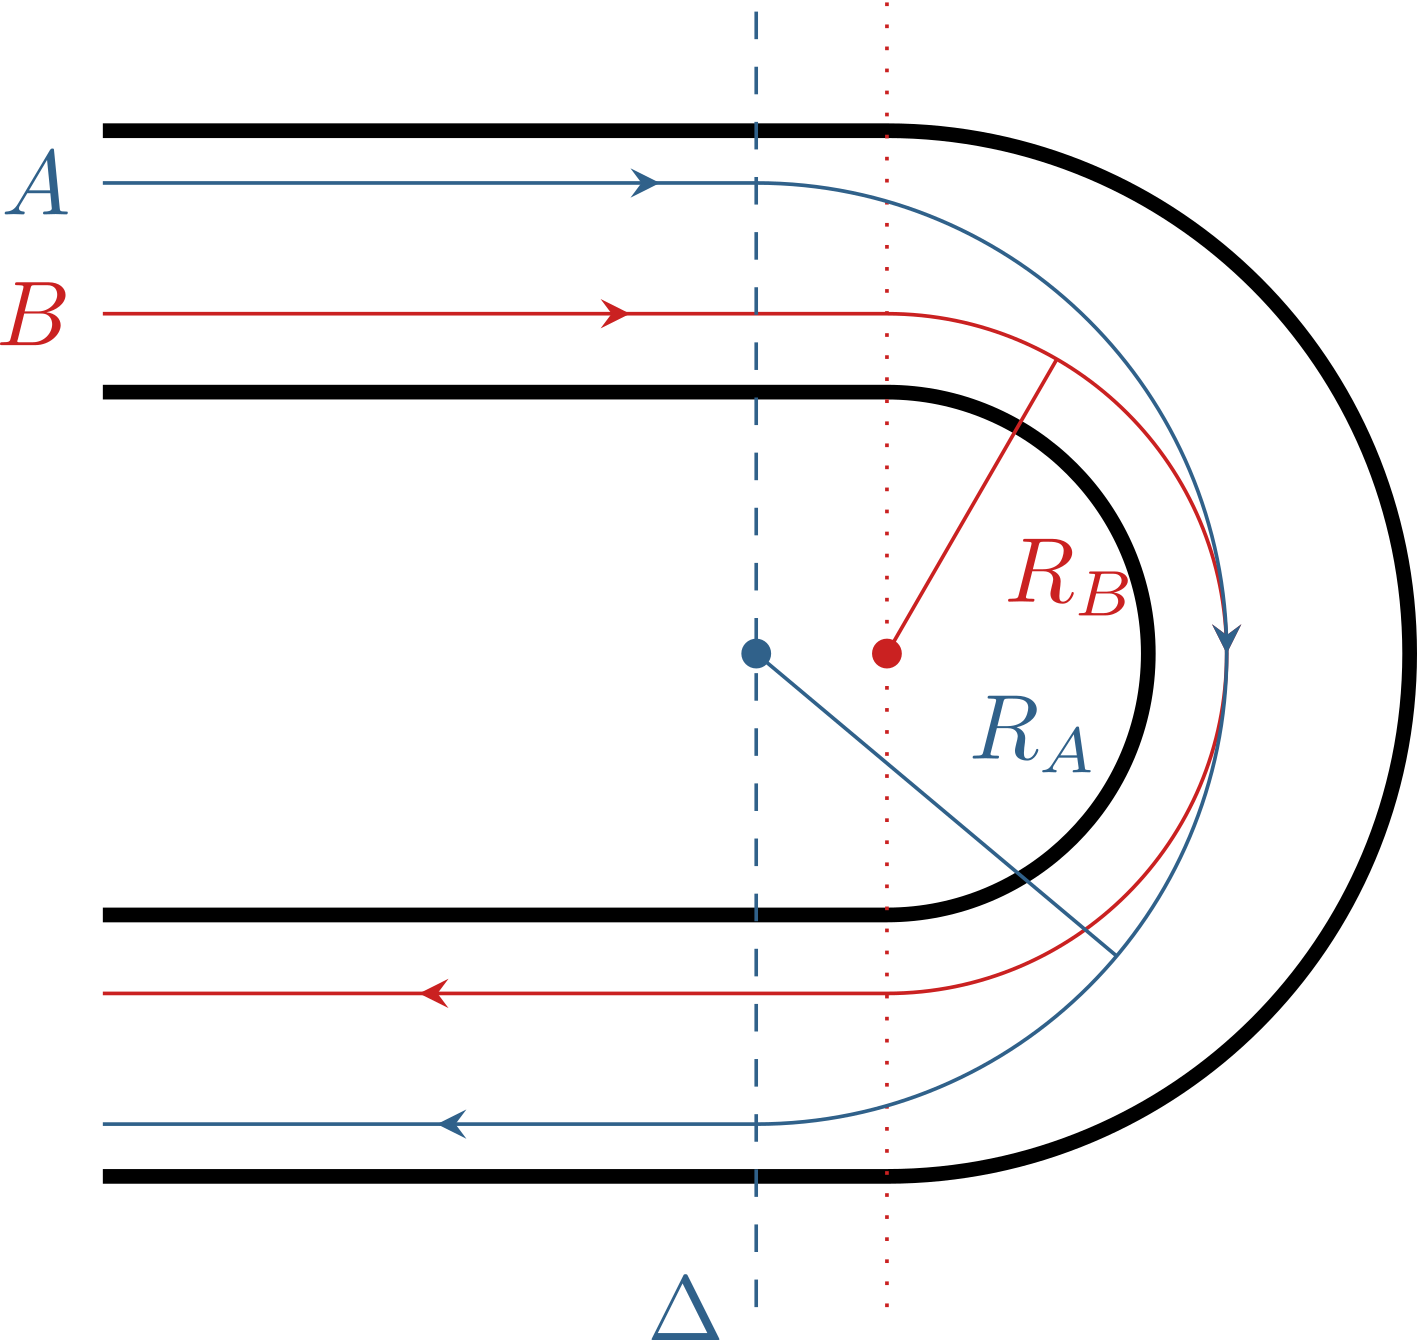
\includegraphics[width=\linewidth]{F1_plain}
		\end{center}
	\end{minipage}
}%

\QR{%
  Déterminer les distances $D_A$ et $D_B$ parcourues par les deux pilotes entre
  leurs deux passages par l'axe $\D$. Que peut-on conclure~?
}{%
  La voiture A d'\textsc{Alonso} entame son virage dès qu'elle passe par
  l'axe $\D$, et parcourt un demi-cercle de longueur
	\[\boxed{D_A = \pi R_A = \SI{283}{m}}\]
  En revanche, la voiture B de \textsc{Button} continue en ligne droite
  sur une distance $R_A-R_B$ avant d'entamer son virage, et parcourt de nouveau
  la même distance en ligne droite avant la sortie du virage. Ainsi,
	\[\boxed{D_B = 2(R_1-R_2) + \pi R_B = \SI{266}{m}}\]
  La voiture B parcourt moins de distance que la voiture A, mais
  \textbf{il est impossible d'en conclure quoi que ce soit} puisqu'on ne
  sait pas si les deux trajectoires sont parcourues à la même vitesse.
}%

\QR{%
  Pour simplifier, on imagine que les deux voitures roulent à des vitesse $v_A$
  et $v_B$ constantes entre leurs deux passages par l'axe $\D$. Déterminer ces
  vitesses, sachant que l'accélération des voitures
  doit rester inférieur à \SI{0.8}{g} sous risque de dérapage. Les
  calculer numériquement.
}{%
  Lorsqu'elles sont sur la partie circulaire de leur trajectoire, parcourue à
  vitesse constante (en norme), l'accélération (en norme) des voitures vaut
	\[a = \frac{v^2}{R} = \num{0.8}g\]
  puisque les pilotes prennent tous les risques. Ainsi,
	\[
		\boxed{v_A = \sqrt{aR_A} = \SI{26.6}{m.s^{-1}}}
		\qet
		\boxed{v_B = \sqrt{aR_B} = \SI{24.3}{m.s^{-1}}}
	\]
}%

\QR{%
  Conclure quant à la meilleure trajectoire des deux.
}{%
  Calculons le temps mis par chacun des pilotes pour passer le virage. On sait
  que
	\[\Dt = \frac{D}{v}\]
  d'où les résultats
	\[
		\boxed{\Dt_A = \SI{10.6}{s}}
		\qet
		\boxed{\Dt_B = \SI{10.9}{s}}
	\]
  Finalement, \textsc{Alonso} va plus vite que \textsc{Button} pour
  parcourir le virage~: \textbf{la meilleure trajectoire est la plus courte des
  deux}, soit ici \textbf{celle la plus large}. À ne pas tenter en vérifiant
  chez soi, mais de quoi briller
  sur Mario Kart…?
}%
\end{document}
